\chapter{Plasticity Basics}
Here we present a general framework of plasticity.

The idealisation of a typical elasto-plastic model can be represented by a frictional device as shown in \figref{fig:idealisation}. The device consists of an elastic spring element that deforms in an elastic manner, the deformation of which can be fully recovered when applied external force becomes zero, and a friction element, which deforms when deformation exceeds a certain limit and its deformation cannot be recovered even when applied external force becomes zero.

Most plastic models are formulated in \textbf{stress space}, or equivalently, \textbf{strain driven}. The task is to determine stress response based on strain input.
\begin{figure}[ht]
\centering
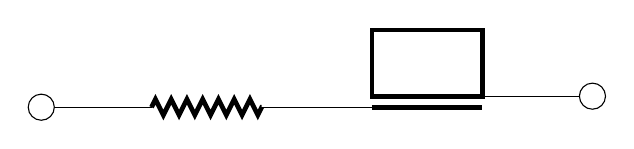
\begin{tikzpicture}[scale=1.4]
\draw(2,0)node[circle,draw,fill=white]{}--(3,0)(4,0)--++(2,0)(5,.1)--++(2,0)node[circle,draw,fill=white]{};
\draw[line width=.6mm](5,0)--++(1,0)(5,.1)rectangle(6,.7);
\draw[line width=.6mm,decorate,decoration={zigzag,segment length=2mm, amplitude=1mm}](3,0)--++(1,0);
\end{tikzpicture}
\caption{idealisation of a typical elasto-plastic model}\label{fig:idealisation}
\end{figure}
\section{Decomposition of Strain}
With the above model, it is clear that total strain $\bvarepsilon$ can be decomposed into two parts, namely recoverable elastic strain $\bvarepsilon^e$ and unrecoverable plastic strain $\bvarepsilon^p$.
\begin{gather}
\bvarepsilon=\bvarepsilon^e+\bvarepsilon^p.
\end{gather}
The elastic part obeys Hooke's law,
\begin{gather}\label{eq:strain_decomposition}
\bsigma=\mb{D}:\bvarepsilon^e=\mb{D}:\left(\bvarepsilon-\bvarepsilon^p\right),
\end{gather}
where $\mb{D}$ is the elastic stiffness moduli.
\section{Yield Function}
To be able to determine whether a given stress state is admissible, the yield function is introduced as the criterion. It is often a scaler--valued function of stress $\bsigma$ and some additional internal variables $\bq$, viz.,
\begin{gather}
f=f\left(\bsigma,~\bq\right).
\end{gather}
By convention, it is defined so that all admissible stress states would lead to $f\leqslant0$ while $f>0$ is not allowed by any means. If $f$ is deemed as a surface in stress space, all admissible stress states shall fall in the volume bounded by $f$. Thus yield function is also called yield surface in some literature, it may further evolve (change of size, location, etc.) with the development of plasticity. Sometimes it is further classified into two types: initial yield surface (when plasticity has not occurred) and subsequent yield surface (when plasticity has developed and is developing).

The internal variables $\bq$ are called history variables.
\section{Flow Rule}
As plastic strain may evolve during the loading/unloading process, it is necessary to know how it evolves, the flow rule is defined as follows.
\begin{gather}
\dot{\bvarepsilon^p}=\gamma\mb{r}\left(\bsigma,~\bq\right),
\end{gather}
where $\gamma$ is a non-negative scalar called the consistency parameter, $\mb{r}=\mb{r}\left(\bsigma,~\bq\right)$ is a tensor--valued function that indicates the direction of plastic flow.

In the context of plasticity, since time $t$ is often not explicitly involved, the dot symbol $\dot{\left(\cdot\right)}$ above a quantity denotes its increment $\dot{\left(\cdot\right)}=\pdfrac{\left(\cdot\right)}{t}\Delta{}t$ for brevity.
\section{Hardening Law}
In order to allow yield function to evolve, internal variables shall be governed by some function, which is defined as hardening law.
\begin{gather}
\dot{\bq}=\gamma\mb{h}\left(\bsigma,~\bq\right),
\end{gather}
where $\mb{h}=\mb{h}\left(\bsigma,~\bq\right)$ is another tensor--valued function that indicates the type of harderning.
\section{Consistency Conditions}
Since $f\ngtr0$ and $\gamma\nless0$, the number of admissible situations is limited:
\begin{itemize}
\item $f<0$ --- elastic loading/unloading
\item $f=0$ and $\dot{f}<0$ --- elastic unloading from yield surface
\item $f=0$ and $\dot{f}=0$ and $\gamma>0$ --- plastic loading
\item $f=0$ and $\dot{f}=0$ and $\gamma=0$ --- neutral loading on current yield surface
\end{itemize}
The above lengthy list can be elegantly characterised by the consistency conditions:
\begin{gather}\label{eq:consistency_condition}
\gamma{}f=0\qquad\text{and}\qquad\gamma\dot{f}=0.
\end{gather}
\section{State Determination}
The yield function, flow rule and hardening law are three elements that complete most plastic models.

For a given strain input $\Delta\varepsilon$ and initial conditions, a general algorithm would possess the following structure.
\begin{breakablealgorithm}
\caption{general state determination algorithm of plastic models}
\begin{algorithmic}[1]
\State freeze plasticity (assume elastic loading/unloading)
\State compute yield function $f$
\If {$f\geqslant0$}
	\State plasticity must develop
	\State compute plastic response
	\State update internal variables
\Else
	\State elastic loading/unloading
	\State compute elastic response
	\State no need to update internal variables
\EndIf
\end{algorithmic}
\end{breakablealgorithm}
\subsection{Local Iteration}
If plasticity must develop, noting that $f=0$, with the assist of \eqsref{eq:strain_decomposition}, $\bsigma$ can be equivalently represented by $\bvarepsilon^p$, there are three unknown variables $\gamma$, $\bvarepsilon^p$ and $\bq$ to be solved subjected to the following three equations.
\begin{gather}
\left\{
\begin{array}{l}
0=f\left(\bvarepsilon^p,~\bq\right),\\
\dot{\bvarepsilon^p}=\gamma\mb{r}\left(\bvarepsilon^p,~\bq\right),\\
\dot{\bq}=\gamma\mb{h}\left(\bvarepsilon^p,~\bq\right).
\end{array}\right.
\end{gather}

Often the above system is nonlinear by construction and needs to be solved with an iterative method. It can be rewritten in a more nonlinear--flavoured style. Let $\mb{x}=\begin{bmatrix}
\gamma&\bvarepsilon^p&\bq
\end{bmatrix}$ denote the local variable vector, and $\mb{R}\left(\gamma,~\bvarepsilon^p,~\bq\right)$ denote the residual of the nonlinear system
\begin{gather}
\mb{R}=\left\{
\begin{array}{l}
f\left(\bvarepsilon^p,~\bq\right),\\
\dot{\bvarepsilon^p}-\gamma\mb{r}\left(\bvarepsilon^p,~\bq\right),\\
\dot{\bq}-\gamma\mb{h}\left(\bvarepsilon^p,~\bq\right).
\end{array}\right.
\end{gather}
The target is to find the solution $\mb{x}$ to $\mb{R}=\mb{0}$ for a prescribed total strain $\bvarepsilon$. The Newton--Raphson method can be adopted with the help of Jacobian $\pdfrac{\mb{R}}{\mb{x}}$. It shall be noted that partial derivatives are used here since fundamentally $\bvarepsilon$ enters the system. It is also a variable which is held constant only at local iteration level.
\subsection{Consistent Tangent Stiffness}
To compute the consistent tangent stiffness, one can start from \eqsref{eq:strain_decomposition},
\begin{gather}
\pdfrac{\bsigma}{\bvarepsilon}=\mb{D}-\mb{D}:\pdfrac{\bvarepsilon^p}{\bvarepsilon}.
\end{gather}

Noting that at equilibrium, local residual shall be zero, viz., $\mb{R}=\mb{0}$. Taking full differentiation leads to
\begin{gather}\label{eq:consistent_stiffness}
\pdfrac{\mb{R}}{\bvarepsilon}+\pdfrac{\mb{R}}{\mb{x}}\pdfrac{\mb{x}}{\bvarepsilon}\equiv\mb{0},
\end{gather}
thus
\begin{gather}
\pdfrac{\mb{x}}{\bvarepsilon}=-\left(\pdfrac{\mb{R}}{\mb{x}}\right)^{-1}\pdfrac{\mb{R}}{\bvarepsilon}.
\end{gather}
The term $\pdfrac{\bvarepsilon^p}{\bvarepsilon}$ can be extracted from $\pdfrac{\mb{x}}{\bvarepsilon}$.

Although not in the closed--form, the above procedure provides a universal approach to compute the consistent tangent stiffness in a highly efficient manner which can be applied to a wide range of plastic models.

Readers who are interested in plasticity theory please refer to \cite{Simo1998} for more formal mathematical formulations.
\section{Some Tensor Quantities}
Here we present some frequently used tensor quantities defined in 3D space.
\subsection{Spherical Stress}
The spherical stress of a stress tensor $\bsigma$ refers to the portion corresponds to an isotropic hydrostatic pressure $p$,
\begin{gather}
p=\dfrac{1}{3}\tr{\bsigma}=\dfrac{1}{3}\sigma_{ii}=\dfrac{1}{3}\left(\sigma_{11}+\sigma_{22}+\sigma_{33}\right).
\end{gather}
The corresponding spherical stress $\mb{p}$ in the Voigt notation is then
\begin{gather}
\mb{p}=p\mb{1}=\begin{bmatrix}p&p&p&0&0&0\end{bmatrix}^\mT.
\end{gather}
In which, $\mb{1}$ is the unit second order tensor.
\begin{gather}
\mb{1}=\begin{bmatrix}1&1&1&0&0&0\end{bmatrix}^\mT.
\end{gather}
\subsection{Deviatoric Stress}
The remaining portion is often known the deviatoric stress, denoted by $\mb{s}$.
\begin{gather}
\mb{s}=\dev{\bsigma}=\bsigma-\mb{p}=\begin{bmatrix}
\sigma_{11}-p\\\sigma_{22}-p\\\sigma_{33}-p\\\sigma_{12}\\\sigma_{23}\\\sigma_{31}
\end{bmatrix}=\begin{bmatrix}
\frac{2}{3}&-\frac{1}{3}&-\frac{1}{3}&&&\\
-\frac{1}{3}&\frac{2}{3}&-\frac{1}{3}&&&\\
-\frac{1}{3}&-\frac{1}{3}&\frac{2}{3}&&&\\
&&&1&&\\
&&&&1&\\
&&&&&1
\end{bmatrix}\begin{bmatrix}
\sigma_{11}\\\sigma_{22}\\\sigma_{33}\\\sigma_{12}\\\sigma_{23}\\\sigma_{31}
\end{bmatrix}.
\end{gather}
In tensor notation,
\begin{gather}
\mb{s}=\mathbb{I}^\text{dev}:\bsigma.
\end{gather}
By simple comparison, one can immediately find
\begin{gather}
\mathbb{I}^\text{dev}=\begin{bmatrix}
\frac{2}{3}&-\frac{1}{3}&-\frac{1}{3}&&&\\
-\frac{1}{3}&\frac{2}{3}&-\frac{1}{3}&&&\\
-\frac{1}{3}&-\frac{1}{3}&\frac{2}{3}&&&\\
&&&1&&\\
&&&&1&\\
&&&&&1
\end{bmatrix}
\end{gather}
is the matrix representation of the fourth order deviatoric operator $\mathbb{I}^\text{dev}$. It must be noted that due to the adoption of the Voigt notation, the matrix representation of $\mathbb{I}^\text{dev}$ is \textbf{not} unique.
The above expression is \textbf{only} valid for stress tensors.

It can be expressed as
\begin{gather}
\mathbb{I}^\text{dev}=\mathbb{I}-\dfrac{1}{3}\mb{1}\otimes\mb{1}.
\end{gather}
\subsection{Volumetric Strain}
It is possible to define the volumetric strain $\varepsilon^v$ to be
\begin{gather}
\varepsilon^v=\tr{\bvarepsilon}=\varepsilon_{ii}=\varepsilon_{11}+\varepsilon_{22}+\varepsilon_{33}.
\end{gather}
In tensor notation, it is
\begin{gather}
\varepsilon^v=\mb{1}:\bvarepsilon.
\end{gather}
\subsection{Deviatoric Strain}
Similarly, the remaining portion of strain is called the deviatoric strain $\bvarepsilon^d$.
\begin{gather}
\be=\bvarepsilon^d=\dev{\bvarepsilon}=\bvarepsilon-\dfrac{\varepsilon^v}{3}\mb{1}=\begin{bmatrix}
\varepsilon_{11}-\frac{\varepsilon^v}{3}\\\varepsilon_{22}-\frac{\varepsilon^v}{3}\\\varepsilon_{33}-\frac{\varepsilon^v}{3}\\2\varepsilon_{12}\\2\varepsilon_{23}\\2\varepsilon_{31}
\end{bmatrix}=\begin{bmatrix}
\frac{2}{3}&-\frac{1}{3}&-\frac{1}{3}&&&\\
-\frac{1}{3}&\frac{2}{3}&-\frac{1}{3}&&&\\
-\frac{1}{3}&-\frac{1}{3}&\frac{2}{3}&&&\\
&&&1&&\\
&&&&1&\\
&&&&&1
\end{bmatrix}\begin{bmatrix}
\varepsilon_{11}\\\varepsilon_{22}\\\varepsilon_{33}\\\gamma_{12}\\\gamma_{23}\\\gamma_{31}
\end{bmatrix}.
\end{gather}
In tensor notation,
\begin{gather}
\be=\bvarepsilon^d=\mathbb{I}^\text{dev}:\bvarepsilon.
\end{gather}
\subsection{Invariants}
For a given symmetric tensor $A_{ij}\in\mathbb{R}^3\times\mathbb{R}^3$, it can explicitly expressed as
\begin{gather}
\mb{A}=
\begin{bmatrix}
A_{11}&A_{12}&A_{31}\\
A_{12}&A_{22}&A_{23}\\
A_{31}&A_{23}&A_{33}
\end{bmatrix}.
\end{gather}
It has three invariants, which can be expressed as
\begin{gather}\label{eq:tensor_invariant}
I_1=\tr{\mb{A}}=A_{11}+A_{22}+A_{33},\\
\begin{split}
I_2&=\dfrac{1}{2}\left(\left(\tr{\mb{A}}\right)^2-\tr{\mb{A}^2}\right)\\
&=A_{11}A_{22}+A_{22}A_{33}+A_{11}A_{33}-A_{12}^2-A_{23}^2-A_{31}^2,
\end{split}\\
I_3=\det{\mb{A}}=A_{11}A_{22}A_{33}+2A_{12}A_{23}A_{31}-A_{11}A_{23}^2-A_{22}A_{31}^2-A_{33}A_{12}^2.
\end{gather}
The three invariants $I_1$, $I_2$ and $I_3$ are in fact functions of eigenvalues of $\mb{A}$.
The are invariant in different eigenspaces since eigenvalues do not change with frame transformation.

The corresponding derivatives with regard to $\mb{A}$ (in Voigt notation) can be computed as
\begin{gather}
	\ddfrac{I_1}{\mb{A}}=\begin{bmatrix}
		1 \\
		1 \\
		1 \\
		0 \\
		0 \\
		0
	\end{bmatrix},\qquad
	\ddfrac{I_2}{\mb{A}}=\begin{bmatrix}
		A_{22}+A_{33} \\
		A_{11}+A_{33} \\
		A_{11}+A_{22} \\
		-2A_{12}      \\
		-2A_{23}      \\
		-2A_{31}
	\end{bmatrix},\qquad
	\ddfrac{I_3}{\mb{A}}=\begin{bmatrix}
		A_{22}A_{33}-A_{23}^2       \\
		A_{11}A_{33}-A_{31}^2       \\
		A_{11}A_{22}-A_{12}^2       \\
		2A_{23}A_{31}-2A_{12}A_{33} \\
		2A_{12}A_{31}-2A_{23}A_{11} \\
		2A_{12}A_{23}-2A_{31}A_{22}
	\end{bmatrix}.
\end{gather}

The above holds for any symmetric tensors.
It thus applies to deviatoric tensors as well.
It is possible to define the deviatoric stress invariants as follows, by denoting $\mb{S}=\mb{A}-\dfrac{I_1}{3}\mb{1}$.
\begin{gather}
J_1=\tr{\mb{S}}=0,\\
\begin{split}
J_2&=\dfrac{1}{2}\left(\left(\tr{\mb{S}}\right)^2-\tr{\mb{S}^2}\right)=-\dfrac{1}{2}\tr{\mb{S}^2}\\
&=S_{11}S_{22}+S_{22}S_{33}+S_{11}S_{33}-A_{12}^2-A_{23}^2-A_{31}^2,\\
&=I_2-\dfrac{1}{3}I_1^2,
\end{split}\\
\begin{split}
J_3&=\det{\mb{S}}\\
&=S_{11}S_{22}S_{33}+2A_{12}A_{23}A_{31}-S_{11}A_{23}^2-S_{22}A_{31}^2-S_{33}A_{12}^2,\\
&=I_3-\dfrac{1}{3}I_1I_2+\dfrac{2}{27}I_1^3.
\end{split}
\end{gather}
In some literature, $J_2$ is defined as $J_2=\dfrac{1}{2}\tr{\mb{S}^2}$.
Clearly, if $J_2$ is an invariant, $-J_2$ is also an invariant.
Depending on the context, either definition may be used.
Readers are encouraged to carry out the above laborious computation to validate the results.
In practice, only a single set of functions needs to be implemented.
When an arbitrary tensor is provided as the input, the corresponding invariants shall be computed.
While a deviatoric tensor is provided, the deviatoric invariants are computed.

In the following, we further provide some explicit expressions for strain and stress tensors.
Although it appears to be confusing, one shall realise the fact that \eqsref{eq:tensor_invariant} applies to any given tensors.
\subsubsection{Stress Invariants}
For a stress tensor expressed in the Voigt notation, namely,
\begin{gather}
\bsigma=\begin{bmatrix}
\sigma_{1}\\\sigma_{2}\\\sigma_{3}\\\sigma_{4}\\\sigma_{5}\\\sigma_{6}
\end{bmatrix}=\begin{bmatrix}
\sigma_{11}\\\sigma_{22}\\\sigma_{33}\\\sigma_{12}\\\sigma_{23}\\\sigma_{31}
\end{bmatrix},
\end{gather}
the invariants can be explicitly written as
\begin{gather}
I_1=\sigma_1+\sigma_2+\sigma_3,\\
I_2=\sigma_1\sigma_2+\sigma_2\sigma_3+\sigma_1\sigma_3-\sigma_4^2-\sigma_5^2-\sigma_6^2,\\
I_3=\sigma_1\sigma_2\sigma_3+2\sigma_4\sigma_5\sigma_6-\sigma_1\sigma_5^2-\sigma_2\sigma_6^2-\sigma_3\sigma_4^2.
\end{gather}
\subsubsection{Strain Invariants}
For a strain tensor expressed in the Voigt notation, namely,
\begin{gather}
\bvarepsilon=\begin{bmatrix}
\varepsilon_{11}\\\varepsilon_{22}\\\varepsilon_{33}\\2\varepsilon_{12}\\2\varepsilon_{23}\\2\varepsilon_{31}
\end{bmatrix}=\begin{bmatrix}
\varepsilon_{1}\\\varepsilon_{2}\\\varepsilon_{3}\\\gamma_{12}\\\gamma_{23}\\\gamma_{31}
\end{bmatrix},
\end{gather}
the invariants can be explicitly written as
\begin{gather}
I_1=\varepsilon_1+\varepsilon_2+\varepsilon_3,\\
I_2=\varepsilon_1\varepsilon_2+\varepsilon_2\varepsilon_3+\varepsilon_1\varepsilon_3-\dfrac{\gamma_{12}^2+\gamma_{23}^2+\gamma_{31}^2}{4},\\
I_3=\varepsilon_1\varepsilon_2\varepsilon_3+\dfrac{\gamma_{12}\gamma_{23}\gamma_{31}}{4}-\dfrac{\varepsilon_1\gamma_{23}^2+\varepsilon_2\gamma_{31}^2+\varepsilon_3\gamma_{12}^2}{4}.
\end{gather}
\subsection{Hooke's Law}
The spherical part and deviatoric part are governed by two material parameters: bulk modulus $K$ and shear modulus $G$, in tensor notation,
\begin{gather}
p=K\varepsilon^v,\qquad\mb{s}=2G\bvarepsilon^d.
\end{gather}
Please note the latter in component form reads
\begin{gather}
\underbrace{\begin{bmatrix}
s_{11}&s_{12}&s_{31}\\
s_{12}&s_{22}&s_{23}\\
s_{31}&s_{23}&s_{33}
\end{bmatrix}}_{\mb{s}}
=
2G
\underbrace{\begin{bmatrix}
\varepsilon^d_{11}&\varepsilon^d_{12}&\varepsilon^d_{31}\\
\varepsilon^d_{12}&\varepsilon^d_{22}&\varepsilon^d_{23}\\
\varepsilon^d_{31}&\varepsilon^d_{23}&\varepsilon^d_{33}
\end{bmatrix}}_{\bvarepsilon^d}.
\end{gather}
The corresponding compressed matrix representation shall be expressed as
\begin{gather}\label{eq:dev_tensor_se}
\underbrace{\begin{bmatrix}
s_{11}\\
s_{22}\\
s_{33}\\
s_{12}\\
s_{23}\\
s_{31}
\end{bmatrix}}_{\mb{s}}
=
2G\underbrace{\begin{bmatrix}
1&&&&&\\
&1&&&&\\
&&1&&&\\
&&&\frac{1}{2}&&\\
&&&&\frac{1}{2}&\\
&&&&&\frac{1}{2}
\end{bmatrix}}_{\mathbb{I}}
\underbrace{\begin{bmatrix}
\varepsilon^d_{11}\\
\varepsilon^d_{22}\\
\varepsilon^d_{33}\\
2\varepsilon^d_{12}\\
2\varepsilon^d_{23}\\
2\varepsilon^d_{31}
\end{bmatrix}}_{\bvarepsilon^d}
=
2G\underbrace{\begin{bmatrix}
\frac{2}{3}&-\frac{1}{3}&-\frac{1}{3}&&&\\
-\frac{1}{3}&\frac{2}{3}&-\frac{1}{3}&&&\\
-\frac{1}{3}&-\frac{1}{3}&\frac{2}{3}&&&\\
&&&\frac{1}{2}&&\\
&&&&\frac{1}{2}&\\
&&&&&\frac{1}{2}
\end{bmatrix}}_{\mathbb{I^\text{dev}}}
\underbrace{\begin{bmatrix}
\varepsilon_{11}\\
\varepsilon_{22}\\
\varepsilon_{33}\\
2\varepsilon_{12}\\
2\varepsilon_{23}\\
2\varepsilon_{31}
\end{bmatrix}}_{\bvarepsilon}.
\end{gather}
In this case, the matrix representation of $\mathbb{I}$ (as well as $\mathbb{I^\text{dev}}$) changes its form since it links strain with stress while in previous examples those unit tensors associate strain with strain, or stress with stress.

This inconsistency is caused by the Voigt notation.
If the Mandel notation is used, the unit tensors are the same for all cases.
Readers are encouraged to derive the above expression using the Mandel notation to gain a better understanding.
One can again refer to \cite{Helnwein2001} for detailed explanation.

After some manipulations, total stress can be expressed by total strain as follows.
\begin{gather}
\begin{split}
\bsigma&=\mb{s}+p\mb{1}\\
&=2G\bvarepsilon^d+K\varepsilon^v\mb{1}\\
&=2G\mathbb{I}^\text{dev}:\bvarepsilon+K\mb{1}\otimes\mb{1}:\bvarepsilon\\
&=\left(2G\mathbb{I}^\text{dev}+K\mb{1}\otimes\mb{1}\right):\bvarepsilon.
\end{split}
\end{gather}
Thus,
\begin{gather}
\mb{D}=2G\mathbb{I}^\text{dev}+K\mb{1}\otimes\mb{1}=2G\mathbb{I}-2G\dfrac{1}{3}\mb{1}\otimes\mb{1}+K\mb{1}\otimes\mb{1}.
\end{gather}

In matrix representation,
\begin{gather}
\mb{D}=2G\begin{bmatrix}
\dfrac{2}{3}&-\dfrac{1}{3}&-\dfrac{1}{3}&\cdot&\cdot&\cdot\\[3mm]
-\dfrac{1}{3}&\dfrac{2}{3}&-\dfrac{1}{3}&\cdot&\cdot&\cdot\\[3mm]
-\dfrac{1}{3}&-\dfrac{1}{3}&\dfrac{2}{3}&\cdot&\cdot&\cdot\\[3mm]
\cdot&\cdot&\cdot&\dfrac{1}{2}&\cdot&\cdot\\[3mm]
\cdot&\cdot&\cdot&\cdot&\dfrac{1}{2}&\cdot\\[3mm]
\cdot&\cdot&\cdot&\cdot&\cdot&\dfrac{1}{2}
\end{bmatrix}+K\begin{bmatrix}
1&1&1&\cdot&\cdot&\cdot\\[3mm]
1&1&1&\cdot&\cdot&\cdot\\[3mm]
1&1&1&\cdot&\cdot&\cdot\\[3mm]
\cdot&\cdot&\cdot&\cdot&\cdot&\cdot\\[3mm]
\cdot&\cdot&\cdot&\cdot&\cdot&\cdot\\[3mm]
\cdot&\cdot&\cdot&\cdot&\cdot&\cdot
\end{bmatrix}.
\end{gather}

Using Lam\'{e}'s constant $\lambda=K-\dfrac{2}{3}G$, $\mb{D}$ can be alternatively expressed as
\begin{gather}
\mb{D}=\begin{bmatrix}
\lambda+2G&\lambda&\lambda&\cdot&\cdot&\cdot\\
\lambda&\lambda+2G&\lambda&\cdot&\cdot&\cdot\\
\lambda&\lambda&\lambda+2G&\cdot&\cdot&\cdot\\
\cdot&\cdot&\cdot&G&\cdot&\cdot\\
\cdot&\cdot&\cdot&\cdot&G&\cdot\\
\cdot&\cdot&\cdot&\cdot&\cdot&G
\end{bmatrix}.
\end{gather}
This form is widely seen in elementary elasticity.
\subsection{Lode Angle}
For some material models, the Haigh--Westergaard stress space may be used. The lode angle is often used to define some parameter that alters the yield surface which may have a special shape on the $\pi$-plane. The lode angle $\theta$ can be defined as
\begin{gather}\label{eq:lode}
\cos\left(3\theta\right)=\dfrac{J_3}{2}\left(\dfrac{3}{J_2}\right)^{1.5},
\end{gather}
where
\begin{gather}
J_2=\dfrac{1}{2}\tr{\bs^2}=\dfrac{1}{2}\norm{\bs}^2,\qquad
J_3=\dfrac{1}{3}\tr{\bs^3}=\det{\bs}
\end{gather}
are the invariants of the deviatoric stress tensor $\bs$.

\eqsref{eq:lode} can be equivalently expressed as
\begin{gather}
\cos\left(3\theta\right)=\dfrac{6^{1.5}}{2}\dfrac{J_3}{\norm{\bs}^3}=\sqrt{54}\dfrac{\det{\bs}}{\norm{\bs}^3}=\sqrt{54}\det{\dfrac{\bs}{\norm{\bs}}}.
\end{gather}

By the chain rule, the derivative of \eqsref{eq:lode} can be expressed as
\begin{gather}\label{eq:dlode}
\ddfrac{\cos\left(3\theta\right)}{\bs}=\dfrac{1}{2}\left(\dfrac{3}{J_2}\right)^{1.5}\ddfrac{J_3}{\bs}-\dfrac{3^{2.5}}{4}\dfrac{J_3}{J_2^{2.5}}\ddfrac{J_2}{\bs}.
\end{gather}
With the assist of
\begin{gather}
\ddfrac{J_2}{\bs}=\bs,\qquad
\ddfrac{J_3}{\bs}=\bs\cdot\bs-\dfrac{2}{3}J_2\mb{1},
\end{gather}
\eqsref{eq:dlode} becomes
\begin{gather}
\begin{split}
\ddfrac{\cos\left(3\theta\right)}{\bs}&=\dfrac{1}{2}\left(\dfrac{3}{J_2}\right)^{1.5}\left(\bs\cdot\bs-\dfrac{2}{3}J_2\mb{1}\right)-\dfrac{3^{2.5}}{4}\dfrac{J_3}{J_2^{2.5}}\bs\\
&=\sqrt{2}\left(\dfrac{3}{2J_2}\right)^{1.5}\left(\bs\cdot\bs-\dfrac{2J_2}{3}\mb{1}-\dfrac{3}{2J_2}J_3\bs\right).
\end{split}
\end{gather}
Denoting $s=\dfrac{2J_2}{3}$, then
\begin{gather}
\ddfrac{\cos\left(3\theta\right)}{\bs}=\sqrt{2}s^{-1.5}\left(\bs\cdot\bs-s\mb{1}-\dfrac{J_3}{s}\bs\right).
\end{gather}